%!TEX program = xelatex
%%%%%%%%%%%%%%%%%%%%%%%这是导言部分的开始%%%%%%%%

%========= 导言部分声明文档的类型=================
\documentclass{article}

%=========导言部分可可以加载宏包=================
\usepackage{amsmath}                % 数学公式排版宏包
\usepackage{amssymb}                % 数学符号命令宏包
\usepackage{amsthm}                 % 数学定理宏包
\usepackage[UTF8]{ctex}             % 中文输入宏包
\usepackage[a4paper]{geometry}      % 页面设置宏包
\usepackage{setspace}               % 行间距宏包
\usepackage{graphicx}               % 图片宏包
\usepackage{listings}               % 代码宏包
\usepackage{color}					% 颜色宏包
\usepackage{xcolor}                 % 颜色处理宏包
\usepackage{float}                  % 浮动对象式样宏包
\usepackage{fontspec}
\usepackage{enumerate}				% 列举编号包

%=========页面设置==============================
\geometry{left=1cm,right=1cm,top=1cm,bottom=2cm}
\onehalfspacing
\setlength\parindent{0em}

%=========代码格式设置============================
\definecolor{dkgreen}{rgb}{0,0.6,0}
\definecolor{gray}{rgb}{0.5,0.5,0.5}
\definecolor{mauve}{rgb}{0.58,0,0.82}
% \setmonofont{Consolas}
\lstset{
	numbers = left, 	
	numberstyle = \color{gray}, 
	keywordstyle = \color{blue},
	commentstyle = \color{dkgreen}, 
	stringstyle = \color{mauve},
	basicstyle = \ttfamily,
	breaklines = true,
	frame = shadowbox, % 阴影效果
	rulesepcolor = \color{ red!20!green!20!blue!20} ,
	escapeinside = ``, % 英文分号中可写入中文
	xleftmargin = 2em,xrightmargin=2em, aboveskip=1em,
	framexleftmargin = 2em
} 

%=========导言部分可以定义标题信息===============
\title{组会报告}
\author{徐益}
\date{\today}
%%%%%%%%%%%%%%%%%%%%%%%这是导言部分的结束%%%%%%%%%

%%%%%%%%%%%%%%%%%%%%%%%这是正文部分的开始%%%%%%%%%
\begin{document}

%=========生成标题================================
\maketitle

%=========开始正文的输入==========================

%===========第一节=================
\section{工作内容}
1. 收数据程序结构化;

2. 编写并测试RZF预编码矩阵生成程序;

3. 根据当前架构修改PHY-MAC对接程序及多线程系统。

%===========第二节=================
\section{data\_collection程序结构化}
\begin{figure}[H]
	\centering
	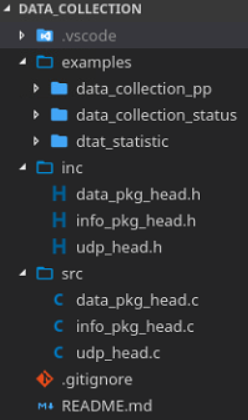
\includegraphics[width = .45\textwidth]{datac.png}
	\caption{data\_collection程序结构}
\end{figure}

%===========第三节=================
\section{编写并测试RZF预编码矩阵生成程序}
\subsection{RZF预编码}
\begin{equation}
W_{RZF}=\beta H(H^H H+\xi I_K)^{-1}
\end{equation}
\subsection{核心函数}
\begin{figure}[H]
	\centering
	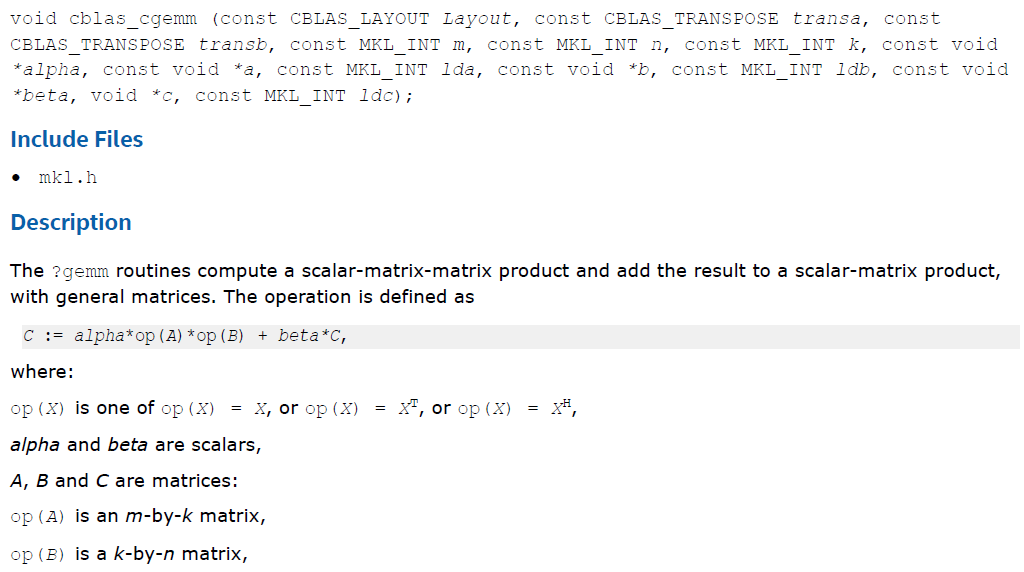
\includegraphics[width = \textwidth]{gemm.png}
	\caption{矩阵运算函数}
\end{figure}
\begin{figure}[H]
	\centering
	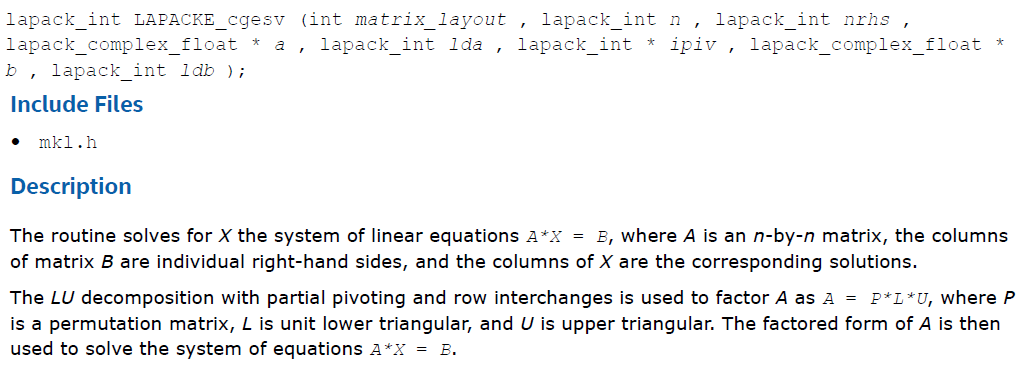
\includegraphics[width = \textwidth]{gesv.png}
	\caption{线性方程求解函数}
\end{figure}
\subsection{表达式变换}
\begin{equation}
	W_{RZF}=H(\frac{1}{\beta} H^H H+\frac{\xi}{\beta} I_K)^{-1}
\end{equation}
\begin{equation}
W_{RZF}=HM^{-1}
\end{equation}
\begin{equation}
W_{RZF}M=H
\end{equation}
\begin{equation}
M^T=W_{RZF}^TH^T
\end{equation}
\subsection{测试结果}
\begin{figure}[H]
	\centering
	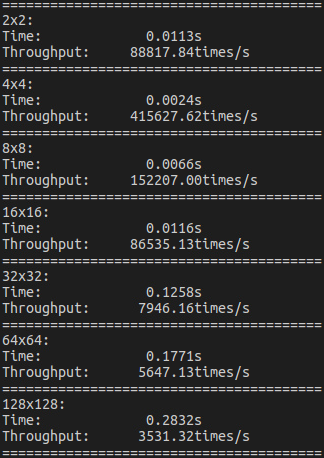
\includegraphics[width = .6\textwidth]{rzf.png}
	\caption{测试结果}
\end{figure}

%===========第四节=================
\section{根据当前架构修改PHY-MAC对接程序及多线程系统}


%===========第五节=================
% \section{5GNR-LDPC报告}


%===========下周计划=================
% \section{下阶段计划}
% 1. 根据当前架构修改与MAC层对接部分;

% 2. 根据当前架构修改多线程系统;

% 3. 参与MIMO信道测试。

\end{document}
%%%%%%%%%%%%%%%%%%%%%%%这是正文部分的结束%%%%%%%%%%%%